\documentclass[12pt,a4paper]{article}
\usepackage[margin=2.5cm]{geometry}
\usepackage[utf8]{inputenc}
\usepackage[
    backend=biber,
    style=apa,
    citestyle=authoryear
]{biblatex}
\setlength{\bibitemsep}{0.5em}
\addbibresource{references.bib}
\usepackage{parskip}
\usepackage{xcolor}
\usepackage{graphicx} % Add this package for including images
\usepackage{hyperref} % Add this package for hyperlinks
\usepackage{caption} % Add this package for caption customization

\title{Multi-core Synergy: A Study of Performance Improvements Utilizing Multi-core Threading}
\author{J. Wolffrom}
\date{\today}

\begin{document}

\maketitle
\newpage

\begin{abstract}

\end{abstract}
\newpage

\tableofcontents
\newpage

\section{Disclosure}

Any and all resources related to- and used in this study can be found here:

\href{https://github.com/X1las/AsSynergy}{https://github.com/X1las/AsSynergy}

Due to the amount of variables that can affect the performance of a CPU, the results of this study should be taken in comparison to each other, and not as a definitive measure of performance. It is encouraged to run the code snippets on your own machine to get a better understanding of the performance improvements that can be achieved with multi-core threading.

\section{Introduction}

According to Moore's Law, the number of transistors on a microchip doubles every two years, leading to an exponential increase in computing power. However, according to \cite{Mattson2014} and \cite{Rauber2023}, this trend dwindled around 2005, as a limit was reached for how many transistors could be placed on a single computer chip without overheating and damaging the circuitry. Even by utilizing the most advanced tricks and optimizations available, the performance improvements we are seeing annually as of 2023 are somewhere around 3.5\% faster CPU's \parencite[p. 11]{Rauber2023} which is a far cry from the 50\% annual increases we were seeing in the early 2000's \parencite[p. 11]{Rauber2023}. 

\begin{quote}
    \textit{\textcolor{darkgray}{Increased clock speeds meant higher heat generation and power consumption, necessitating more robust cooling solutions and improved power management techniques. The quest for ever-higher clock speeds eventually reached a plateau due to these limitations, leading to a shift in CPU design principles.}} - \parencite{mscodes} 
\end{quote}

As a result of the processing speed ceiling, the focus has shifted from increasing the clock speeds of CPUs to adding more computational units to them. This has led to the rise in multi-core processors, which contain multiple processing units on a single chip, often referred to as "cores". These cores can execute multiple orders simultaneiously, which can lead to significant performance improvements in software applications. However, a discrepancy can be found in the communities that rely on these improvements.

\begin{quote}
    \textit{\textcolor{darkgray}{While there are some PC games that love CPUs with a dozen or more cores, they’re few and far between. 
    Instead, finding an 8-core, 16-thread processor with a high clock speed and a lot of L3 Cache is going to get you further than just adding more CPU cores to the equation. }} 
    - \parencite{Thomas2025}
\end{quote}

Within the gaming communities we're seeing a trend of diminishing returns, whereas what we should be seeing is an equivalance. There is a concensus that multi-core threading is the future of software development, and it has been for several years now, even as far back as 2005 \parencite{mscodes}, so the question is what's holding us back?

\subsection{The Problem Area}

If multi-core threading is the future, then it is essential to understand why it is not delivering the expected performance improvements it has the potential to deliver. \parencite[p. 12]{Rauber2023} mentions that simulations have shown that superscalar processors with up to four functional units yield substantial benefits over the use of a single functional unit. So in theory, it would seem there is a great potential to gain from utilizing multiple cores. Some of it has been utilized according to \textcite{Thomas2025}, as we are talking about 8-cores as opposed to one, but it has taken us well over 20 years to get to this point.

As such, this study aims to address this question of why multi-code optimization is so difficult to accomplish, if and/or how it can be improved, and what the potential benefits of doing so are. In addition, we wish to bring to light the concept of multi-core threading or processing as a whole, seeing as it has slipped out of the public's eye in recent years. Now, more than ever, with the rise of machine learning and AI, we need to be able to utilize the full potential of our hardware.

\subsubsection{Research Question}

This being said, there are limits to what can be achieved in such a short study, therefore we will be focusing heavily on the theory behind multi-core computing and how to get startet with it. 

The research question that we will be addressing is then as follows:

\begin{quote}
    \textit{What are the challenges of multi-core optimization, and how can they be overcome?}
\end{quote}

This question can then be further broken down into the following sub-questions:

\begin{itemize}
    \item What does the standard architecture of a CPU look like? Is there one?
    \item What is a thread, and what is a processor?
    \item What frameworks are commonly used for multi-core threading?
    \item What are the challenges of multi-core threading, and how can they be overcome?
\end{itemize}

These questions serve as a guide for the study and will help to structure the research process, beginning with a review of the literature on the topic.

\section{Limitations}

This study is limited in scope to just a handful of programming languages, and even in that case we will just be delving into the details of Python. This is due to the fact that Python isn't necessarily the best language in terms of performance, but is one of the slowest in terms of execution time. This makes python an exceptional candidate for multi-core threading, as it stands to gain the most from it.

As such, the primary focus will be the theory behind multi-core processing in python with a few examples of how to implement it. We will be looking at how languages such as C, Java, and C\# handle multi-core processing, but we will not be going into detail on how to implement it in those languages. The focus will be strictly on comparisons for the sake of understanding key concepts like parallelism and concurrency.

In addition to the limits of programming languages, we will also be limiting the range of operating systems to just Windows and Linux. This is due to the fact that these share the same range of common chipsets as opposed to MacOS, which keeps to a very small range of chipsets. This is not to say that MacOS is not capable of multi-core processing, but rather that most of the practical applications of multi-core processing are applied to Windows and Linux systems.

\section{Terminology}

For the purpose of this paper, we will be using a lot of terminology that refers to the different sub-components of a computer. We expect the reader to have a basic understanding of what a computer is, and a general overview of its components, such as knowing what a CPU is and what role it plays. 

The term \textbf{core} refers to a single processing unit that is housen within a CPU, which will occur frequently in this paper. The term \textbf{thread} and \textbf{process} are often used interchangeably when going over the CPU architecture, but threads are generally smaller and are often used to refer to single tasks of which a process could contain many. This is not to be confused with a \textbf{processor} which is a kind of processing unit that is smaller in size than a core, and is often used to refer to the physical chip that is used to execute the orders.

\section{Synchronous and Asynchronous systems}

When looking at computing with multi-core systems it is important to understand the difference between a synchronous and asynchronous system. In general, when we talk about systems that use a single processing unit we usually always talk of a synchronous system, as orders are executed in order. When we scale this order up to several processing units on the same chipset we have what is referred to as a multicore processor, which is the focal point of this study. This multicore processor can then either be synchronous in order to keep to the order of executions that computers are used to, or we can choose to make it asynchronous, allowing all processing units to execute somewhat independently of each other. 

The reality of synchronous and asynchronous systems is that they are not entirely separate. They are often used in conjunction with each other, as we need levels of synchronization in order to access shared resources between different cores. Simple tasks such as reading and writing to memory is determined by whether another core is using that memory at the same time, further complicating the matter.

\subsubsection{Subroutines and Coroutines}

In order to understand asynchronous systems, it's important to note both subroutines and coroutines. 

Subroutines are the standard way of executing tasks in traditional programming, where the order of execution is determined by the order of which commands are written in the code. These are often known as Functions in programming languages, and are executed in a inear fashion, exiting once they finish executing. This makes then quite similar to coroutines, as they share the same functionality, except for the the ability to suspend their execution, also known by the 'yield' and 'resume' keywords. 

This means that coroutines can be used to execute tasks in a non-linear fashion, allowing for more flexibility in the order of executions. Whether or not we have a coroutine defined as the target to 'yield' to also determines whether we are working with synchronous or asynchronous systems. 'yield'ing to a coroutine means that we are working with dependencies, pausing the execution of a program to wait for a result from another coroutine. 

For an example, look at the following python snippet:
\begin{verbatim}

import asyncio

async def main():
    print('Hello ...')
    await asyncio.sleep(1)
    print('... World!')

asyncio.run(main())
\end{verbatim}

Which defines an asynchronous main function, or a coroutime that will print "Hello World" interspaced by one second. This shows the prominent 'yield' functionality. If we gave the function a target to yield to, we would in turn make the code synchronous in nature.

\subsection{Threading}

The reason why subroutines and coroutines are important to understand is because they relate quite heavily to how threads operate. 

Threading is a way of executing multiple different tasks at the same time in a computer operating system. Every program on a computer intrinsically define at least one thread of operations they want the operating system to execute. This is often referred to as the main thread, and is the thread that is executed first when a program is started, which can then spawn sub-threads to execute other tasks. The OS then handles what order threads are executed in using what is known as a "Scheduler", this scheduler is then also responsible for 'Suspending' threads to make it seem like all programs are executed concurrently. 

This process of suspending threads is what allows for the illusion of concurrency, allowing the operating system to seemingly execute multiple threads at the same time by switching back and forth rapidly between tasks. This is known as "context switching", and is a key feature of modern operating systems, making even a single core processing system capable of multi-tasking.

This is not to be confused with multi-core processing, which is the ability to execute multiple threads at the same time with different cores. This is where the real performance improvements come from, as we can execute multiple tasks at the same time without having to switch as often.

\section{Parallelism}
This ability to execute multiple tasks simultaneously with multiple cores is known as "parallelism". In this section we will be looking at notable terms and concepts that are important to understand when working with multi-core systems.
\subsection{Degree of Parallelism}

In the field of parallel systems architecture we often talk about the degree of parallelism a system is capable of. This is a measure of how many tasks can be executed at the same time, and is often used to describe the performance improvements that a parallel system provides.

This, in turn, coincides with the concept of "Potential Parallelism", which is the theoretical maximum degree of parallelism that a system can achieve. This is often used to describe the performance improvements that a parallel system can provide, and is often used as a benchmark for comparing different systems.

\subsubsection{Parallel Execution Time (PET)}

In this context of degrees of parallelism, we often use measures such as "Parallel Execution Time" (PET) to quantitatively describe the time it takes for a parallel system to execute a given task. 

This execution time is measured across all functional units, or cores of a system, and can be used to give a tangible measure of the running time of a parallel program. This means that waiting times for memory fetching, writing and plain idle times are included in the measure.

In terms of coding with multi-core threading, this means that "scheduling" time is included in the measure as well, as this is the time it takes for the operating system to assign tasks to different cores. This is important to note, as it means that the performance improvements of a parallel system are not just determined by the number of cores, but also by the efficiency of the scheduling algorithm used by the operating system.

\subsubsection{Load Balancing}

The term "Load Balancing" refers to the standard process of distributing tasks across multiple cores in a parallel system, such that tasks are executed equally across all cores. This is important to ensure that all cores are utilized effectively, and that no single core is overloaded with tasks while others are idle.

To this, it is important to note that not all cores are created equal, and that in terms of cpu-architecture we see a lot of variation with "Performance" and "Optional" cores. Performance cores are designed to handle heavy workloads, while optional cores are designed to handle lighter workloads. This means that load balancing is not just about distributing tasks evenly across all cores, but also about ensuring that the right tasks are assigned to the right cores. 

Even within the same core type we can see a lot of variation in terms of performance, as some cores are designed to handle specific tasks better than others. This is known as "heterogeneous computing", and is an important consideration when designing parallel systems, but as mentioned earlier, in this paper we will only deal with intel x64 architecture.

\subsubsection{Idle Time}

The time a processor cannot do anything useful but wait for more work.

\section{Memory}
\subsection{Shared Memory}

Memory organization where the machine shares memory for all threads.

Synchronization plays a heavy role, for example by keeping threads from reading files before another has written to them.

Often connected to the term "Thread".

\subsection{Memory Access Time (MAT)}

Add content if applicable.

\section{Schedulers}

Add content if applicable.

\section{TRIN Model}

Add content if applicable.

\section{State of the Field}
\subsection{Python}

As it stands, Python is one of the most popular programming languages in the field of computer science. It is widely used in a variety of applications due to its simplicity and ease of use. However, it is an interpreted language, which means that it is not as fast as compiled languages like C or C++. In fact it is written in C, which is a compiled language. This means that in places it keeps the speed of C by pre-compiling certain commands, but in other places it is slower than C, with up to 10 times the execution in difference.

This is important due to the way Python handles multi-core threading. By default, Python comes pre-installed with threading and asynchronous libraries, which allow for the use of multiple threads in a program, however the presence of the Global Interpreter Lock (GIL) means that only one core will be in use at any time. This means that the performance improvements of multi-core threading are not easily accessed, but by using libraries such as 'multiprocessing' or 'numpy', we can bypass the GIL using some of the same utilities in C. This allows us to use multiple cores in a program, but it is not as easy to implement as it is in other languages.

\subsection{Java}

Java comes with a built-in threading library, which allows for the use of multiple threads in a program, managed by the Java Virtual Machine (JVM). Usually this is accomplished by inheritance, designating a class as a thread, allowing it to use common threading methods such as sleep (suspension) and join (synchronization). This means that Java is able to utilize multiple cores in a program by use of their own scheduler, and the performance improvements are easily accessible. However, this is not without its drawbacks, as the JVM is an interpreted language, which means that it is not as fast as compiled languages like C or C++. In addition, the JVM is not as efficient as other languages when it comes to memory management, which can lead to performance issues in large programs. 

\subsection{C\#}

C\# is a compiled language that is part of the C language family like Python, however where it differs is its striking resemblance to Java. It is a high-level language that is designed to be easy to use and understand, gathering a lot of attention due to its usage in the Unity game engine as well as developers transitioning from other languages. It is therefore a prime candidate for multi-core processing optimization as Java developers come potentially pre-equipped with a solid foundation of threading, as well as new game developers looking for performance improvements.

The way C\# handles multi-core threading is not the same as Java, as it provides a library to assign tasks to threads, which in turn are managed by the operating system's scheduler. This means that C\# is able to utilize multiple cores in a program, but it is not as easy to implement as it is in Java. However, C\# does have some advantages over Java when it comes to performance, as it is a compiled language and therefore faster than Java. In addition, C\# has a more efficient memory management system than Java, which can lead to performance improvements in large programs.

\subsection{C}

C, unlike the previous mentions, is a low-level programming language. It is a compiled language that is designed to be fast and efficient, making it a popular choice for system programming and embedded systems. C is often used in applications where performance is critical, such as operating systems, device drivers, and high-performance computing, as well as game engines. It is therefore a prime candidate for multi-core processing optimization, as wherever C is used in practice it is often done so with performance in mind.

C provides a library for multi-core threading called Posix, labeling their way of threading as 'pthreads' or 'POSIX threads'. This library is a standard for multi-core threading in C, and comes pre-installed with unix systems such as Linux in the GCC compiler used for this study.

\section{Data Collection}

Before we get into the benchmarks of the different programming languages, it is important to disclose that the data was collected on a computer running Ubuntu 24.04.2 LTS with an intel Core i5-4460 CPU @ 3.2GHz, with 4 cores and 4 threads. The time measured was done so with various clocking methods depending on the programming language over the course of 5 runs, with the average time being taken as the final result. The code snippets used for the benchmarks can be found in the appendix.

To begin with, we clocked the time it took to execute a simple count from 1 to 1 billion in the various languages to get a frame of references. This proved especially difficult for Java, as the JIL converts commonly used methods to bytecode to optimize the execution time. This meant that to get a proper benchmark we had to disable the JIT compiler by using the '-Xint' flag, which in turn made the execution time of Java significantly slower than the other languages, with the exception of Python.

\newpage
\section{Results}

As expected, the results of running the code snippets in multiple cores were significant performance increases, as comared to the single core. This makes sense, as evidently four cores are faster than one, however some of these results were quite surprising.

\begin{figure}[!htb]
    \centering
    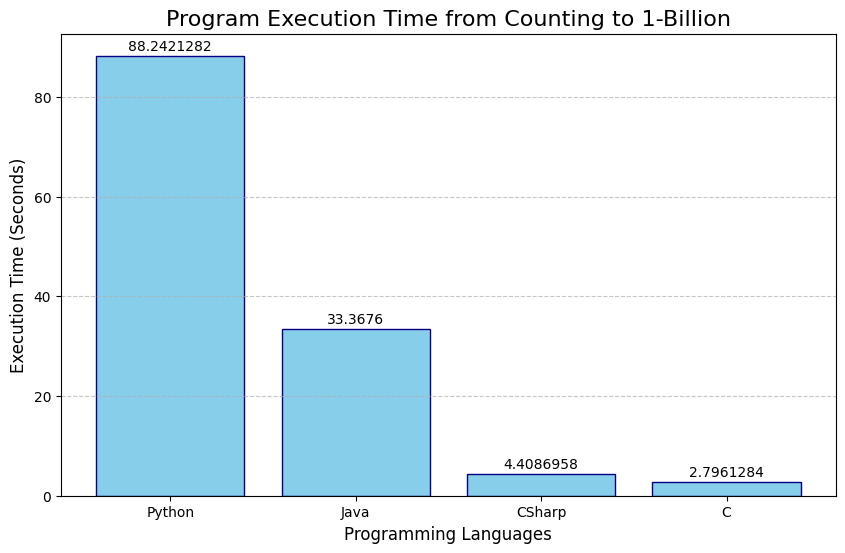
\includegraphics[width=0.8\textwidth]{../sync_records/sync_exec_times.png}
    \captionsetup{font=tiny, justification=centering}
    \caption{Execution time comparison of different programming languages running synchronously when counting from 1 to 1-billion.}
    \label{fig:sync-exec-times}
\end{figure}


The synchronous execution results above benchmark the time it took to compute the same task in each of the language. We saw expected results within most of the languages, with python having an average run time of 88 seconds, Java at 33, C\# 4 and C at a little less than 3 seconds. There was not much to note in these results, other than Java operating surprisingly slow when not using the JIT compiler.


\begin{figure}[!htb]
    \centering
    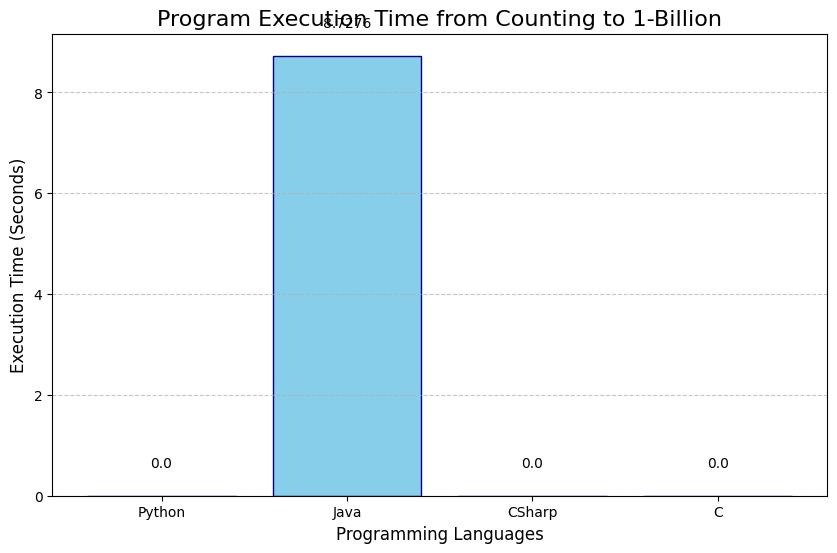
\includegraphics[width=0.8\textwidth]{../async_records/async_exec_times.png}
    \captionsetup{font=tiny, justification=centering}
    \caption{Execution time comparison of different programming languages running asynchronously with multi-threading when counting from 1 to 1-billion.}
    \label{fig:async-exec-times}
\end{figure}

The asynchronous execution results reveal a great deal about the efficiency of the different programming when using multiple cores. Python was able to achieve a time of 43 seconds on average which amounts to a little more than twice the performance increase. Java was able to achieve an astounding 8.7 seconds, a little less than 4 times the performance increase.

\newpage
\section{Discussion}

Include thoughts about other programming languages.

\newpage
\section{Conclusion}

Add content if applicable.

\newpage
\section{References}
\printbibliography
% Ensure Biber is run to resolve undefined references

\clearpage
\appendix

\section{Asynchronous Run-time Snippets}

\subsection{C Code Execution Times} 

\begin{figure}[htbp]
    \centering
    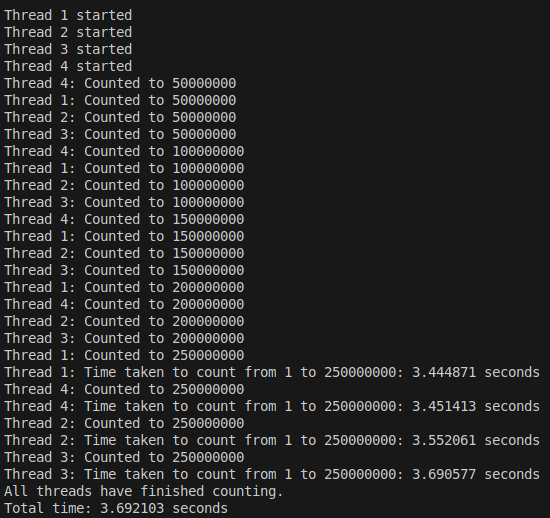
\includegraphics[width=0.8\textwidth]{../async_records/results_c/result_1.png}
    \caption{First run of asynchronous C code execution.}
    \label{fig:C-async-runtime-1}
\end{figure}

\begin{figure}[htbp]
    \centering
    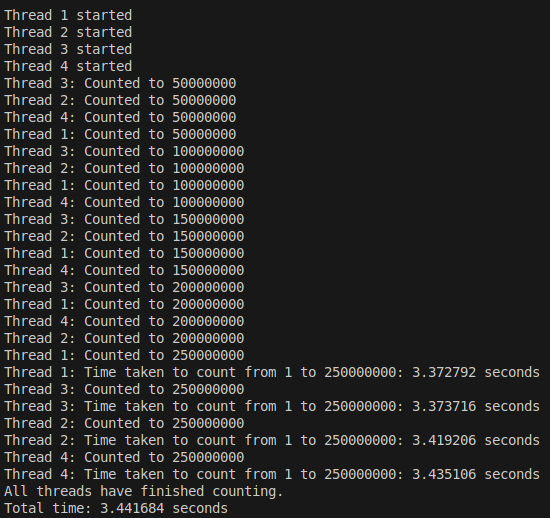
\includegraphics[width=0.8\textwidth]{../async_records/results_c/result_2.png}
    \caption{Second run of asynchronous C code execution.}
    \label{fig:C-async-runtime-2}
\end{figure}

\begin{figure}[htbp]
    \centering
    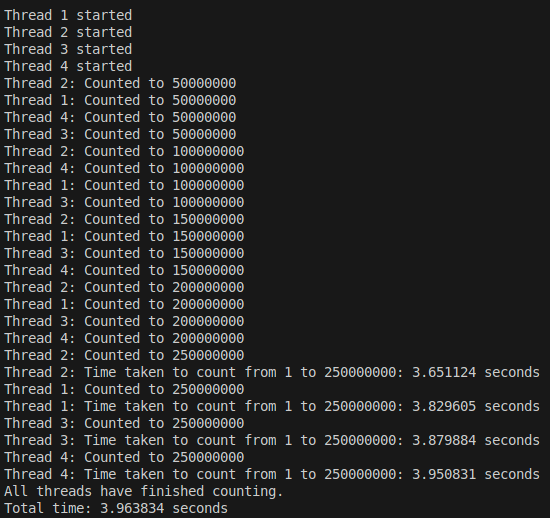
\includegraphics[width=0.8\textwidth]{../async_records/results_c/result_3.png}
    \caption{Third run of asynchronous C code execution.}
    \label{fig:C-async-runtime-3}
\end{figure}

\begin{figure}[htbp]
    \centering
    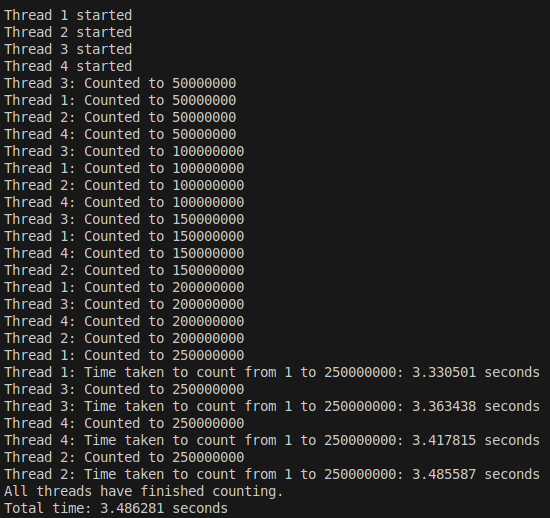
\includegraphics[width=0.8\textwidth]{../async_records/results_c/result_4.png}
    \caption{Fourth run of asynchronous C code execution.}
    \label{fig:C-async-runtime-4}
\end{figure}

\begin{figure}[htbp]
    \centering
    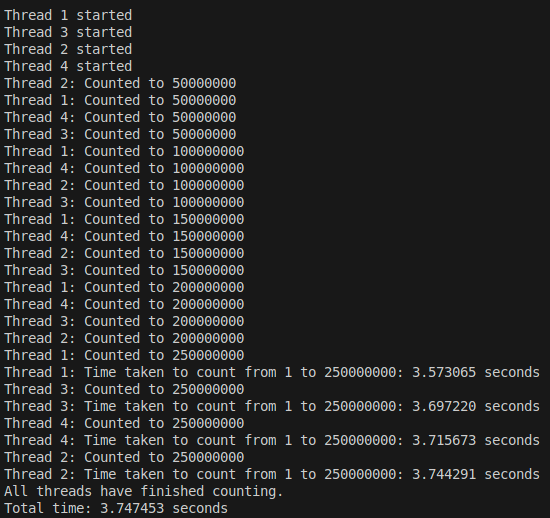
\includegraphics[width=0.8\textwidth]{../async_records/results_c/result_5.png}
    \caption{Fifth run of asynchronous C code execution.}
    \label{fig:C-async-runtime-5}
\end{figure}

\clearpage
\subsection{C-Sharp Code Execution Times} 

\begin{figure}[htbp]
    \centering
    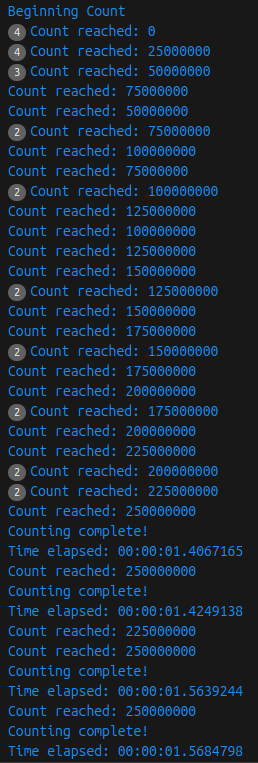
\includegraphics[width=0.8\textwidth]{../async_records/results_cs/result_1.png}
    \caption{First run of asynchronous C-Sharp code execution.}
    \label{fig:C-Sharp-async-runtime-1}
\end{figure}

\begin{figure}[htbp]
    \centering
    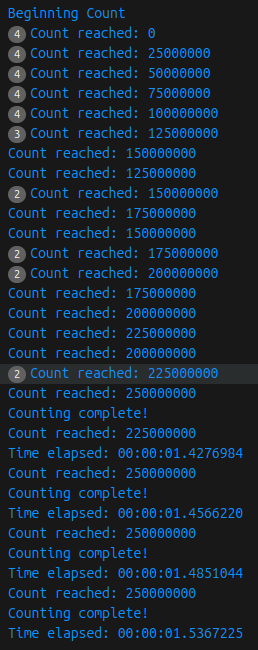
\includegraphics[width=0.8\textwidth]{../async_records/results_cs/result_2.png}
    \caption{Second run of asynchronous C-Sharp code execution.}
    \label{fig:C-Sharp-async-runtime-2}
\end{figure}

\begin{figure}[htbp]
    \centering
    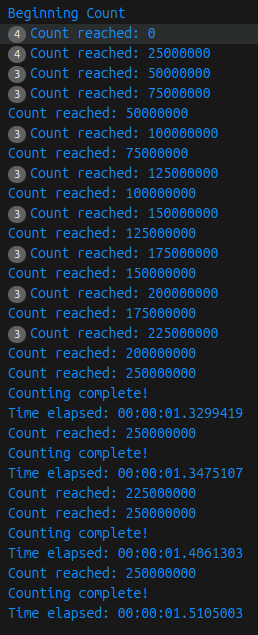
\includegraphics[width=0.8\textwidth]{../async_records/results_cs/result_3.png}
    \caption{Third run of asynchronous C-Sharp code execution.}
    \label{fig:C-Sharp-async-runtime-3}
\end{figure}

\begin{figure}[htbp]
    \centering
    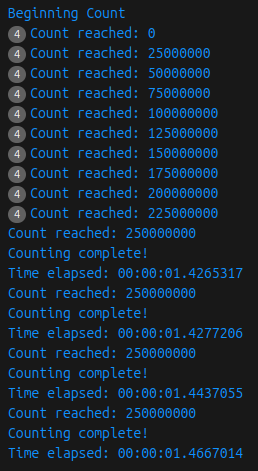
\includegraphics[width=0.8\textwidth]{../async_records/results_cs/result_4.png}
    \caption{Fourth run of asynchronous C-Sharp code execution.}
    \label{fig:C-Sharp-async-runtime-4}
\end{figure}

\begin{figure}[htbp]
    \centering
    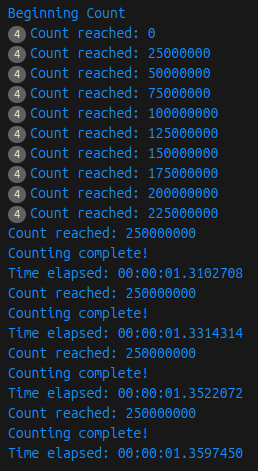
\includegraphics[width=0.8\textwidth]{../async_records/results_cs/result_5.png}
    \caption{Fifth run of asynchronous C-Sharp code execution.}
    \label{fig:C-Sharp-async-runtime-5}
\end{figure}

\clearpage
\subsection{Java Execution Times} 

\begin{figure}[htbp]
    \centering
    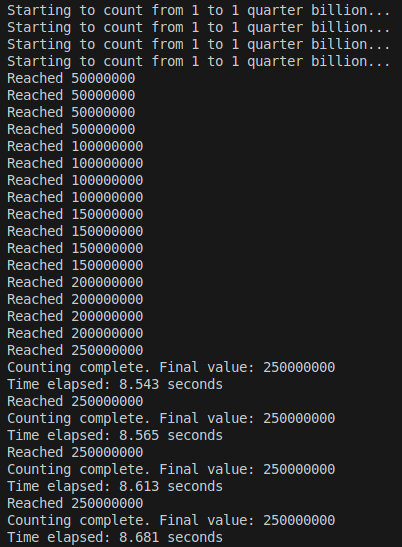
\includegraphics[width=0.8\textwidth]{../async_records/results_java/result_1.png}
    \caption{First run of asynchronous Java code execution.}
    \label{fig:Java-async-runtime-1}
\end{figure}

\begin{figure}[htbp]
    \centering
    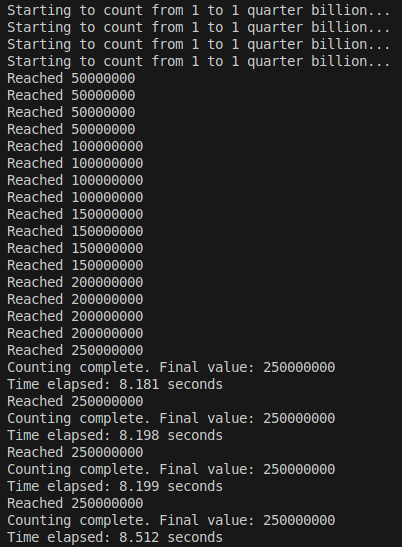
\includegraphics[width=0.8\textwidth]{../async_records/results_java/result_2.png}
    \caption{Second run of asynchronous Java code execution.}
    \label{fig:Java-async-runtime-2}
\end{figure}

\begin{figure}[htbp]
    \centering
    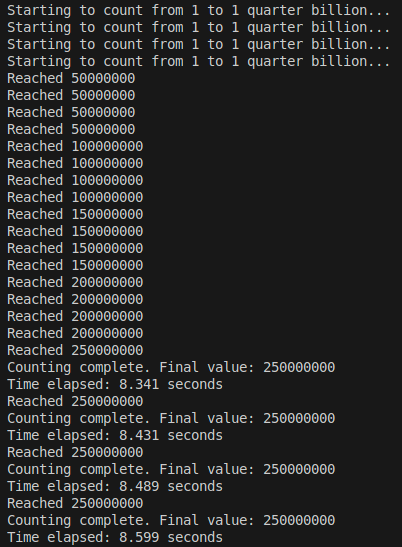
\includegraphics[width=0.8\textwidth]{../async_records/results_java/result_3.png}
    \caption{Third run of asynchronous Java code execution.}
    \label{fig:Java-async-runtime-3}
\end{figure}

\begin{figure}[htbp]
    \centering
    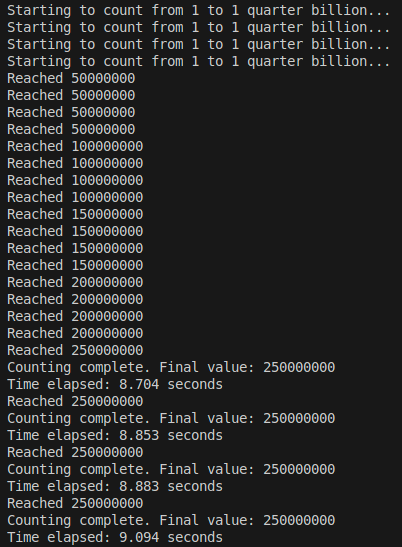
\includegraphics[width=0.8\textwidth]{../async_records/results_java/result_4.png}
    \caption{Fourth run of asynchronous Java code execution.}
    \label{fig:Java-async-runtime-4}
\end{figure}

\begin{figure}[htbp]
    \centering
    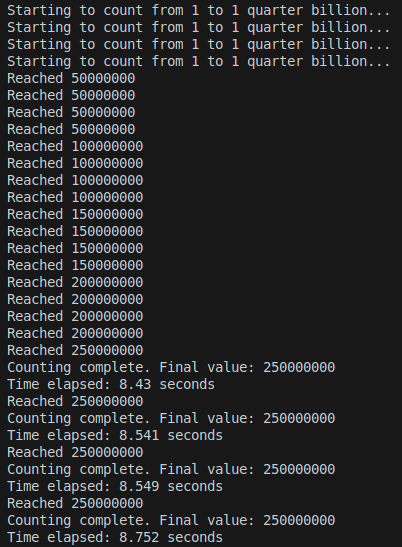
\includegraphics[width=0.8\textwidth]{../async_records/results_java/result_5.png}
    \caption{Fifth run of asynchronous Java code execution.}
    \label{fig:Java-async-runtime-5}
\end{figure}

\clearpage
\subsection{Python Execution Times} 

\begin{figure}[htbp]
    \centering
    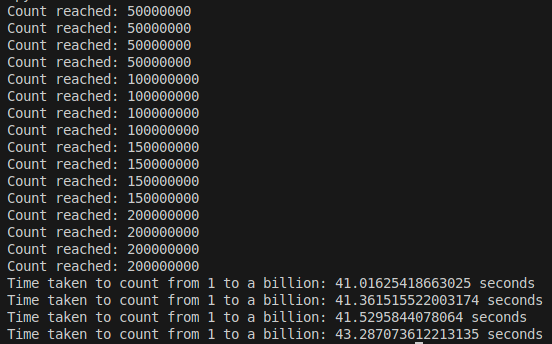
\includegraphics[width=0.8\textwidth]{../async_records/results_python/result_1.png}
    \caption{First run of asynchronous Python code execution.}
    \label{fig:Python-async-runtime-1}
\end{figure}

\begin{figure}[htbp]
    \centering
    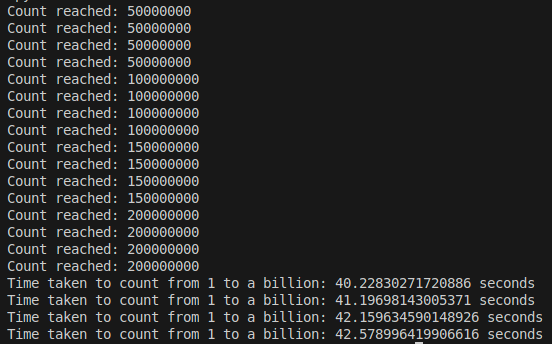
\includegraphics[width=0.8\textwidth]{../async_records/results_python/result_2.png}
    \caption{Second run of asynchronous Python code execution.}
    \label{fig:Python-async-runtime-2}
\end{figure}

\begin{figure}[htbp]
    \centering
    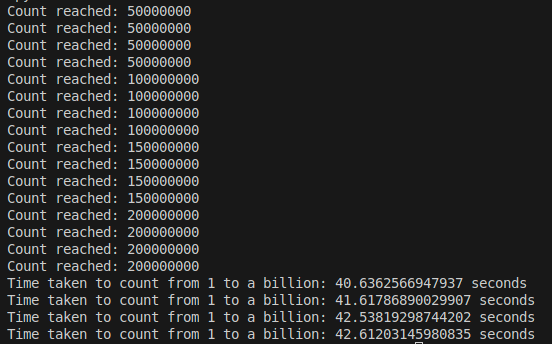
\includegraphics[width=0.8\textwidth]{../async_records/results_python/result_3.png}
    \caption{Third run of asynchronous Python code execution.}
    \label{fig:Python-async-runtime-3}
\end{figure}

\begin{figure}[htbp]
    \centering
    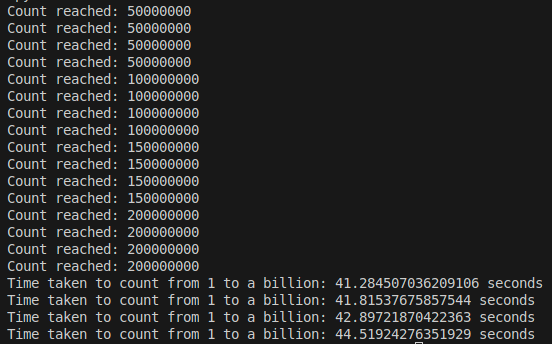
\includegraphics[width=0.8\textwidth]{../async_records/results_python/result_4.png}
    \caption{Fourth run of asynchronous Python code execution.}
    \label{fig:Python-async-runtime-4}
\end{figure}

\begin{figure}[htbp]
    \centering
    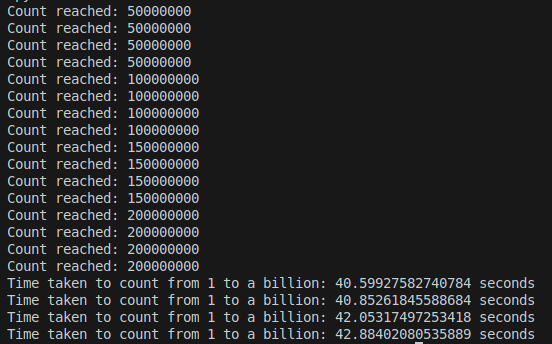
\includegraphics[width=0.8\textwidth]{../async_records/results_python/result_5.png}
    \caption{Fifth run of asynchronous Python code execution.}
    \label{fig:Python-async-runtime-5}
\end{figure}

\clearpage
\section{Synchronous Run-time Snippets}

\subsection{C Code Execution Times} 

\begin{figure}[htbp]
    \centering
    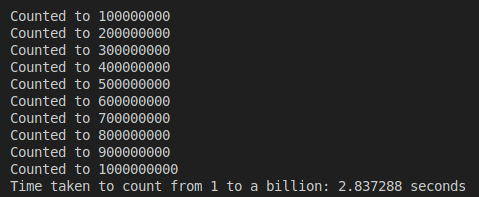
\includegraphics[width=0.8\textwidth]{../sync_records/results_c/result_1.png}
    \caption{First run of synchronous C code execution.}
    \label{fig:C-runtime-1}
\end{figure}

\begin{figure}[htbp]
    \centering
    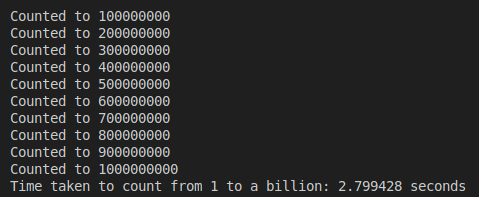
\includegraphics[width=0.8\textwidth]{../sync_records/results_c/result_2.png}
    \caption{Second run of synchronous C code execution.}
    \label{fig:C-runtime-2}
\end{figure}

\begin{figure}[htbp]
    \centering
    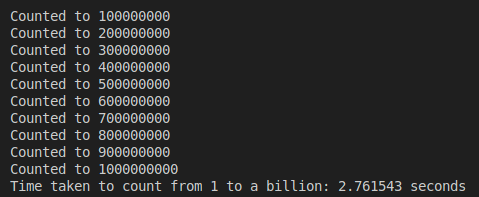
\includegraphics[width=0.8\textwidth]{../sync_records/results_c/result_3.png}
    \caption{Third run of synchronous C code execution.}
    \label{fig:C-runtime-3}
\end{figure}

\begin{figure}[htbp]
    \centering
    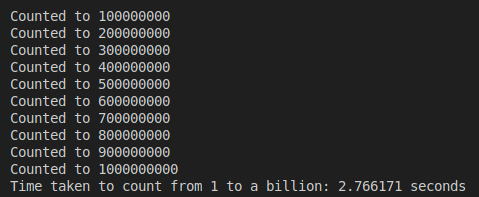
\includegraphics[width=0.8\textwidth]{../sync_records/results_c/result_4.png}
    \caption{Fourth run of synchronous C code execution.}
    \label{fig:C-runtime-4}
\end{figure}

\begin{figure}[htbp]
    \centering
    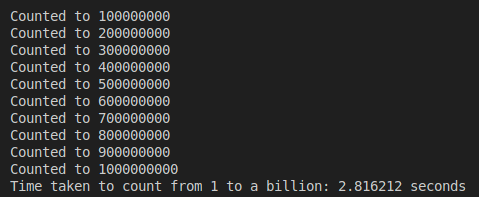
\includegraphics[width=0.8\textwidth]{../sync_records/results_c/result_5.png}
    \caption{Fifth run of synchronous C code execution.}
    \label{fig:C-runtime-5}
\end{figure}

\clearpage
\subsection{C-Sharp Code Execution Times} 

\begin{figure}[htbp]
    \centering
    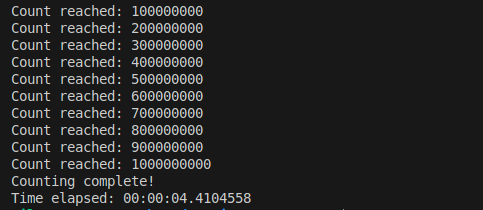
\includegraphics[width=0.8\textwidth]{../sync_records/results_cs/result_1.png}
    \caption{First run of synchronous C-Sharp code execution.}
    \label{fig:C-Sharp-runtime-1}
\end{figure}

\begin{figure}[htbp]
    \centering
    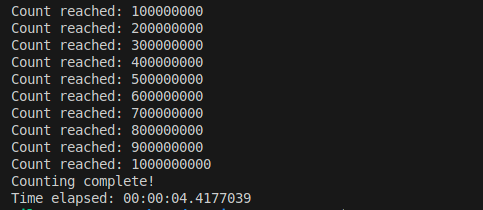
\includegraphics[width=0.8\textwidth]{../sync_records/results_cs/result_2.png}
    \caption{Second run of synchronous C-Sharp code execution.}
    \label{fig:C-Sharp-runtime-2}
\end{figure}

\begin{figure}[htbp]
    \centering
    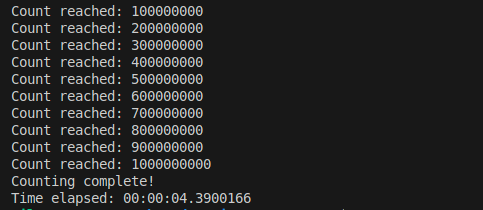
\includegraphics[width=0.8\textwidth]{../sync_records/results_cs/result_3.png}
    \caption{Third run of synchronous C-Sharp code execution.}
    \label{fig:C-Sharp-runtime-3}
\end{figure}

\begin{figure}[htbp]
    \centering
    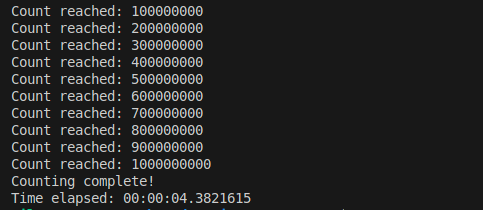
\includegraphics[width=0.8\textwidth]{../sync_records/results_cs/result_4.png}
    \caption{Fourth run of synchronous C-Sharp code execution.}
    \label{fig:C-Sharp-runtime-4}
\end{figure}

\begin{figure}[htbp]
    \centering
    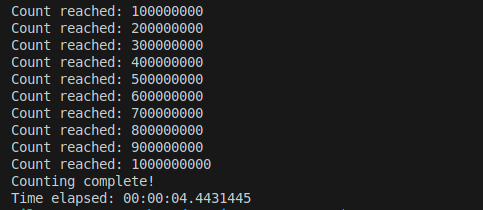
\includegraphics[width=0.8\textwidth]{../sync_records/results_cs/result_5.png}
    \caption{Fifth run of synchronous C-Sharp code execution.}
    \label{fig:C-Sharp-runtime-5}
\end{figure}

\clearpage
\subsection{Java Execution Times} 

\begin{figure}[htbp]
    \centering
    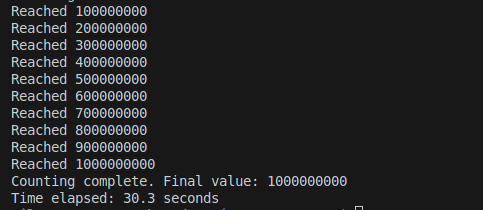
\includegraphics[width=0.8\textwidth]{../sync_records/results_java/result_1.png}
    \caption{First run of synchronous Java code execution.}
    \label{fig:Java-runtime-1}
\end{figure}

\begin{figure}[htbp]
    \centering
    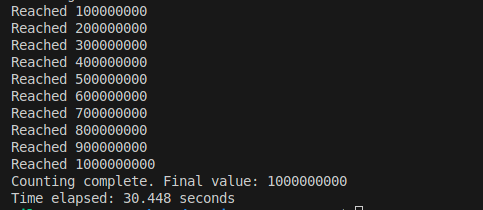
\includegraphics[width=0.8\textwidth]{../sync_records/results_java/result_2.png}
    \caption{Second run of synchronous Java code execution.}
    \label{fig:Java-runtime-2}
\end{figure}

\begin{figure}[htbp]
    \centering
    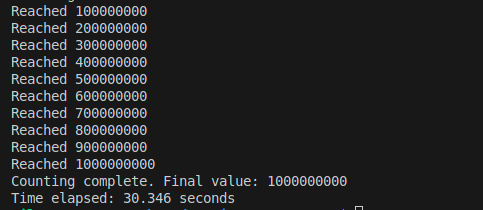
\includegraphics[width=0.8\textwidth]{../sync_records/results_java/result_3.png}
    \caption{Third run of synchronous Java code execution.}
    \label{fig:Java-runtime-3}
\end{figure}

\begin{figure}[htbp]
    \centering
    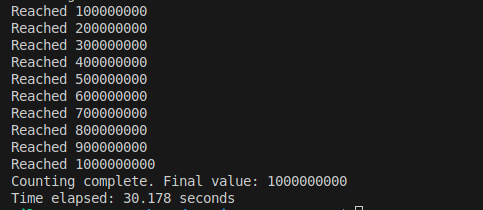
\includegraphics[width=0.8\textwidth]{../sync_records/results_java/result_4.png}
    \caption{Fourth run of synchronous Java code execution.}
    \label{fig:Java-runtime-4}
\end{figure}

\begin{figure}[htbp]
    \centering
    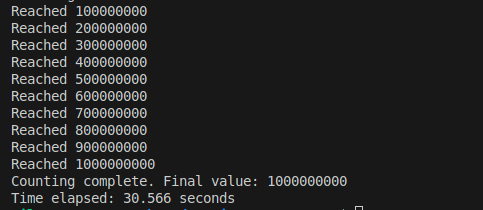
\includegraphics[width=0.8\textwidth]{../sync_records/results_java/result_5.png}
    \caption{Fifth run of synchronous Java code execution.}
    \label{fig:Java-runtime-5}
\end{figure}

\clearpage
\subsection{Python Execution Times} 

\begin{figure}[htbp]
    \centering
    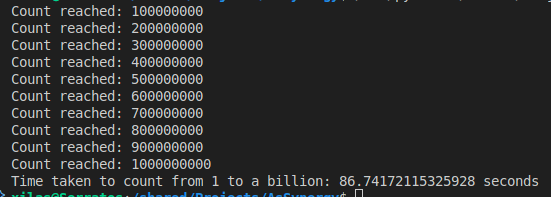
\includegraphics[width=0.8\textwidth]{../sync_records/results_python/result_1.png}
    \caption{First run of synchronous Python code execution.}
    \label{fig:Python-runtime-1}
\end{figure}

\begin{figure}[htbp]
    \centering
    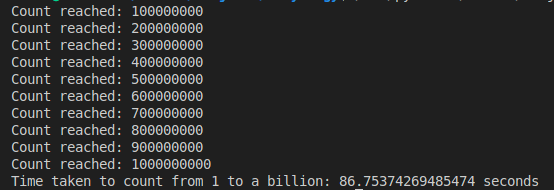
\includegraphics[width=0.8\textwidth]{../sync_records/results_python/result_2.png}
    \caption{Second run of synchronous Python code execution.}
    \label{fig:Python-runtime-2}
\end{figure}

\begin{figure}[htbp]
    \centering
    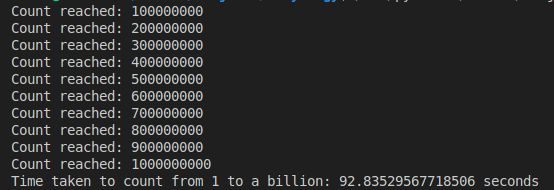
\includegraphics[width=0.8\textwidth]{../sync_records/results_python/result_3.png}
    \caption{Third run of synchronous Python code execution.}
    \label{fig:Python-runtime-3}
\end{figure}

\begin{figure}[htbp]
    \centering
    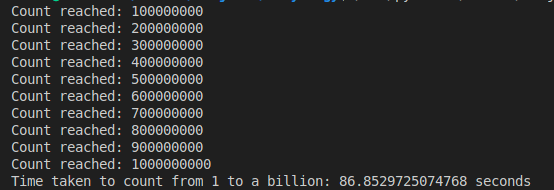
\includegraphics[width=0.8\textwidth]{../sync_records/results_python/result_4.png}
    \caption{Fourth run of synchronous Python code execution.}
    \label{fig:Python-runtime-4}
\end{figure}

\begin{figure}[htbp]
    \centering
    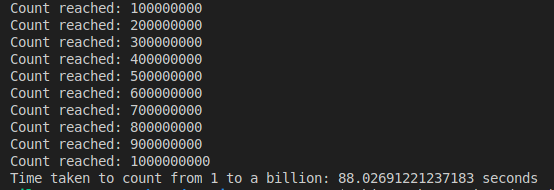
\includegraphics[width=0.8\textwidth]{../sync_records/results_python/result_5.png}
    \caption{Fifth run of synchronous Python code execution.}
    \label{fig:Python-runtime-5}
\end{figure}

\end{document}